\documentclass[10pt, a4paper,spanish]{article}
\usepackage[utf8]{inputenc}

\usepackage{varwidth}
\usepackage{graphicx}

\usepackage[T1]{fontenc} % Use 8-bit encoding that has 256 glyphs
\usepackage{microtype} % Slightly tweak font spacing for aesthetics

\usepackage[hmarginratio=1:1,top=32mm,columnsep=20pt]{geometry} % Document margins
\usepackage[hang, small,labelfont=bf,up,textfont=it,up]{caption} % Custom captions under/above floats in tables or figures
\usepackage{float} % Required for tables and figures in the multi-column environment - they need to be placed in specific locations with the [H] (e.g. \begin{table}[H])
\usepackage{hyperref} % For hyperlinks in the PDF

\usepackage{abstract} % Allows abstract customization
\renewcommand{\abstractnamefont}{\normalfont\bfseries} % Set the "Abstract" text to bold
\renewcommand{\abstracttextfont}{\normalfont\small\itshape} % Set the abstract itself to small italic text

\usepackage{titlesec} % Allows customization of titles
\renewcommand\thesection{\Roman{section}} % Roman numerals for the sections
\renewcommand\thesubsection{\Roman{subsection}} % Roman numerals for subsections
\titleformat{\section}[block]{\large\scshape\centering}{\thesection.}{1em}{} % Change the look of the section titles
\titleformat{\subsection}[block]{\large}{\thesubsection.}{1em}{} % Change the look of the section titles

\usepackage{fancyhdr} % Headers and footers
\pagestyle{fancy} % All pages have headers and footers
\fancyhead{} % Blank out the default header
\fancyfoot{} % Blank out the default footer
\fancyhead[C]{ Marzo 2016 $\bullet$ JumpVa $\bullet$ Análisis de la Aplicación} % Custom header text
\fancyfoot[RO,LE]{\thepage} % Custom footer text

%----------------------------------------------------------------------------------------
%	TITLE SECTION
%----------------------------------------------------------------------------------------

\title{\vspace{-15mm}\fontsize{24pt}{10pt}\selectfont\textbf{Análisis de la Aplicación}} % Article title

\author{
\large
\textsc{Alberto Amigo Alonso\textsubscript{25\%}}\\[2mm] % Your name
\textsc{Sergio Delgado Álvarez\textsubscript{25\%}}\\[2mm] % Your name
\textsc{Sergio García Prado\textsubscript{25\%}}\\[2mm] % Your name
\textsc{Oscar Fernández Angulo\textsubscript{25\%}}\\[2mm] % Your name
\normalsize Universidad de Valladolid \\ % Your institution
\vspace{-5mm}
}
\date{}

%----------------------------------------------------------------------------------------

\begin{document}

	\maketitle % Insert title

	\thispagestyle{fancy} % All pages have headers and footers

%----------------------------------------------------------------------------------------
%	ABSTRACT
%----------------------------------------------------------------------------------------

	\begin{abstract}
		\noindent Servicio web destinado a permitir a remitentes y destinatarios ofertar envíos para que los transportistas sean capaces de encontrarlos permitiendo a todos los usuarios monitorizarlos.
	\end{abstract}

%----------------------------------------------------------------------------------------
%	TEXT
%----------------------------------------------------------------------------------------
	\section{Especificación de requisitos:}

		\paragraph{}
		Requisitos funcionales: El sistema deberá...

			\begin{itemize}
				\item registrar nuevos usuarios.
				\item reconocer el rol de cada usuario.
				\item crear un nuevo envío.
				\item buscar un envío en su historial.
				\item cambiar el estado de los envíos.
				\item permitir al usuario puntuar los envíos.
				\item guardar un historial de los envíos (información).
				\item permitir a los usuarios consultar el estado de los envíos.
				\item actualizar el progreso de los envíos.
				\item permitir a los transportistas pujar por un envío.
				\item permitir a los usuarios añadir hitos a un envío.
				\item asegurar que todos los usuarios están previamente identificados en el sistema para poder acceder a cualquier función.
				\item notificar al usuario nuevas incidencias en los envíos.
				\item permitir a "los que envían" consultar el historial de los transportistas relacionados con el envío.
				\item permitir a "los que envían" puntuar al transportista que ha realizado su envío.
				\item permitir a los transportistas realizar una oferta para un evento.
				\item pedir una confimación para realizar una oferta.
				\item pedir una confimación para asignar un envío.
				\item permitir al transportista buscar nuevos envíos.
			\end{itemize}

			\paragraph{}
			Requisitos no funcionales: El sistema deberá...

				\begin{itemize}
					\item usar una base de datos como medio de almacenamiento.
					\item permitir hacer login a los usuarios que están en la base de datos.
				\end{itemize}
	\section{Casos de uso:}


		\begin{figure}[H]
			\centering
				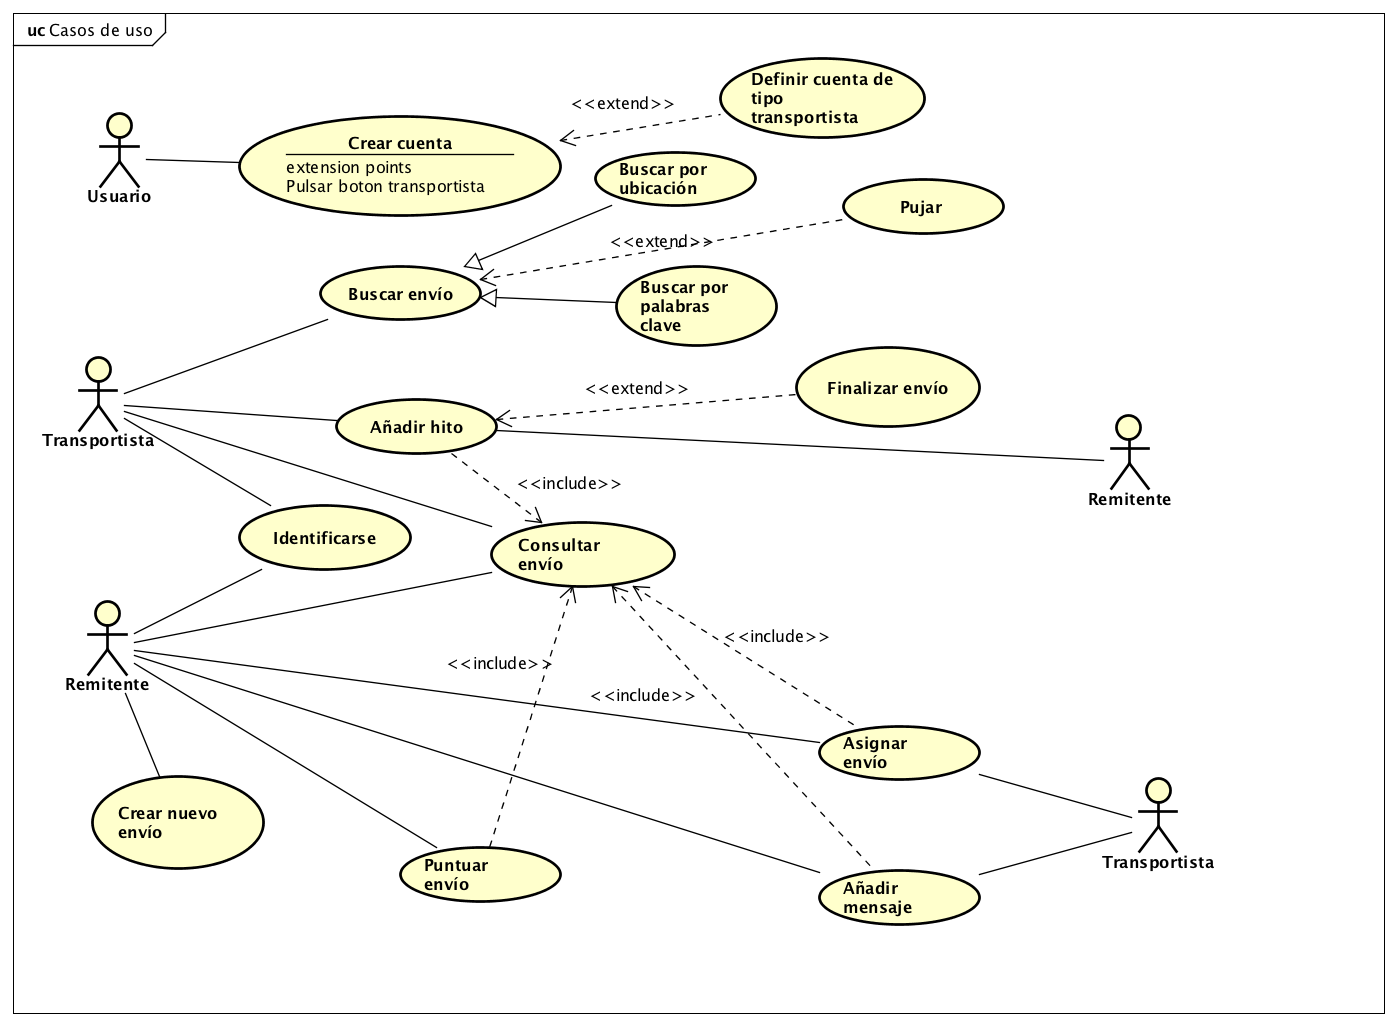
\includegraphics[width=\textwidth]{astah/casos_de_uso.png}
		\end{figure}

		\begin{figure}[H]
			\centering
				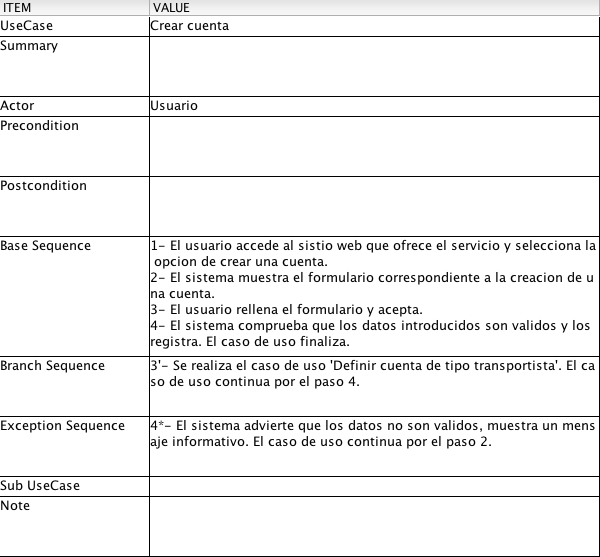
\includegraphics[width=0.75\textwidth]{astah/use_case_crear_cuenta.png}
		\end{figure}

		\begin{figure}[H]
			\centering
				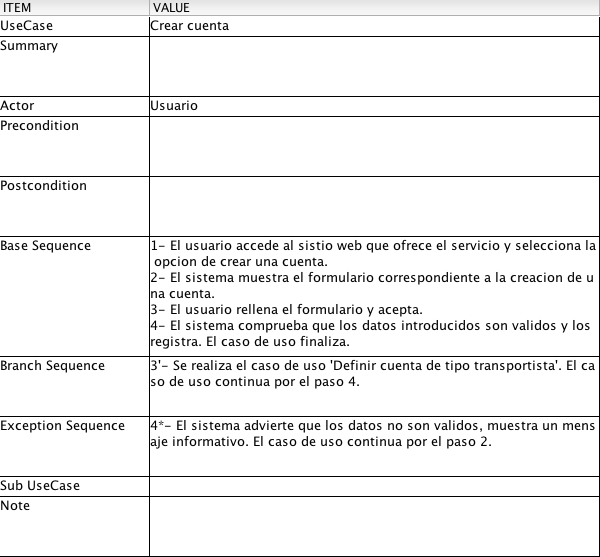
\includegraphics[width=0.75\textwidth]{astah/use_case_crear_cuenta.png}
		\end{figure}

		\begin{figure}[H]
			\centering
				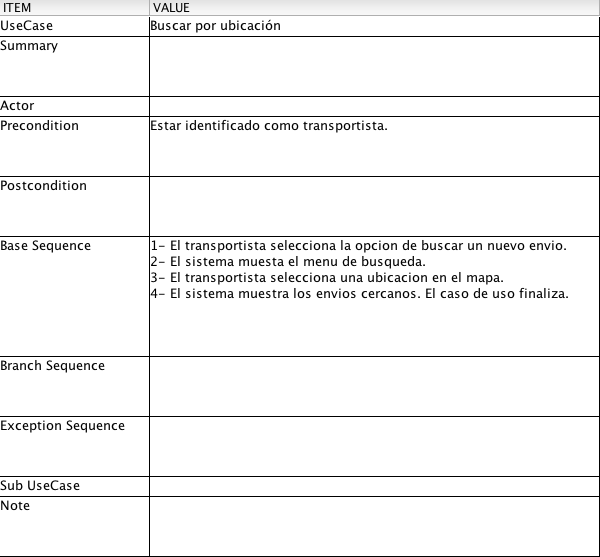
\includegraphics[width=0.75\textwidth]{astah/use_case_buscar_ubicacion.png}
		\end{figure}

		\begin{figure}[H]
			\centering
				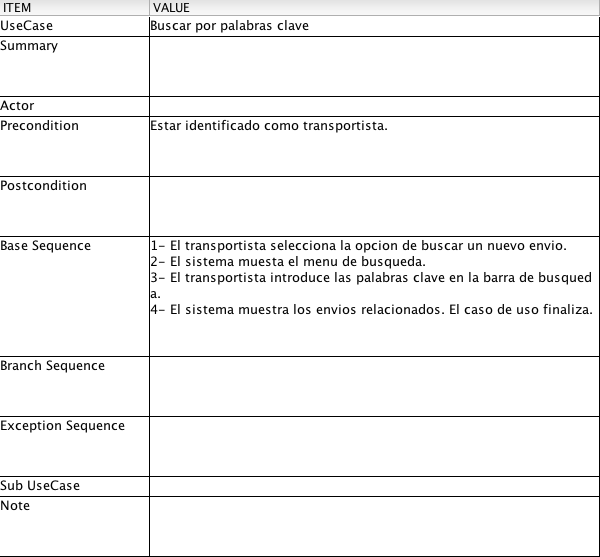
\includegraphics[width=0.75\textwidth]{astah/use_case_buscar_palabras_clave.png}
		\end{figure}

		\begin{figure}[H]
			\centering
				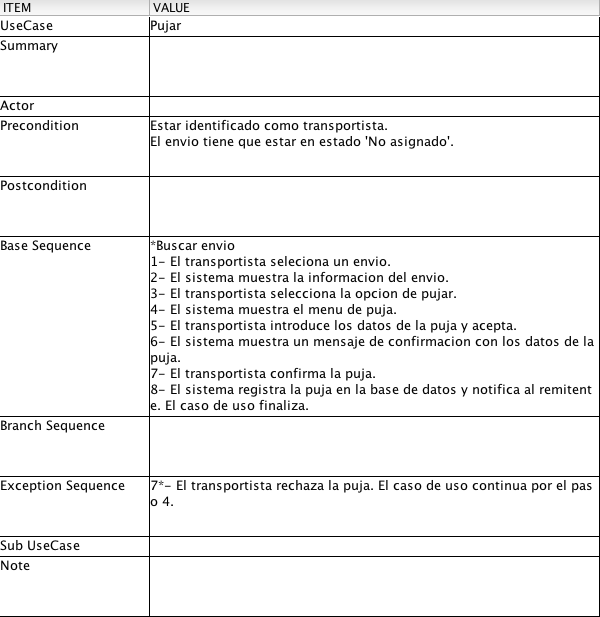
\includegraphics[width=0.75\textwidth]{astah/use_case_pujar.png}
		\end{figure}

		\begin{figure}[H]
			\centering
				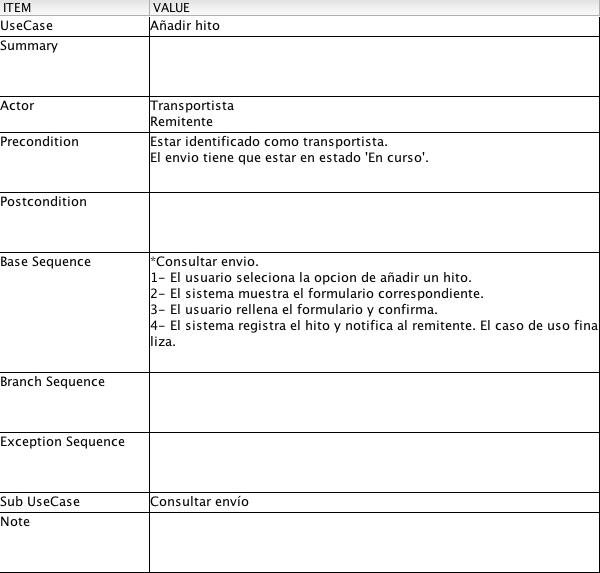
\includegraphics[width=0.75\textwidth]{astah/use_case_anadir_hito.png}
		\end{figure}

		\begin{figure}[H]
			\centering
				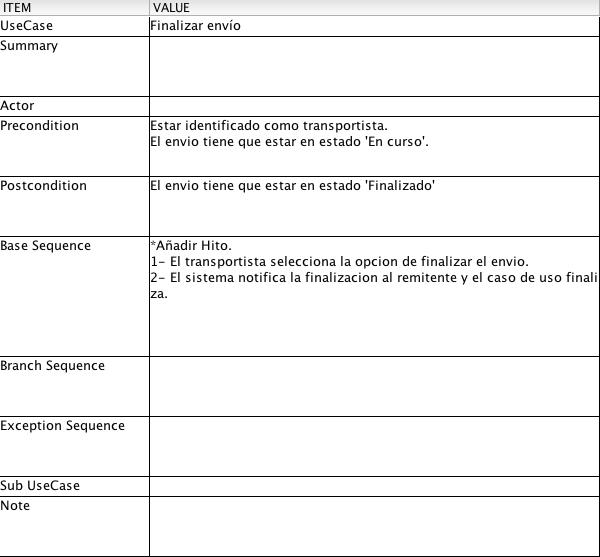
\includegraphics[width=0.75\textwidth]{astah/use_case_finalizar_envio.png}
		\end{figure}

		\begin{figure}[H]
			\centering
				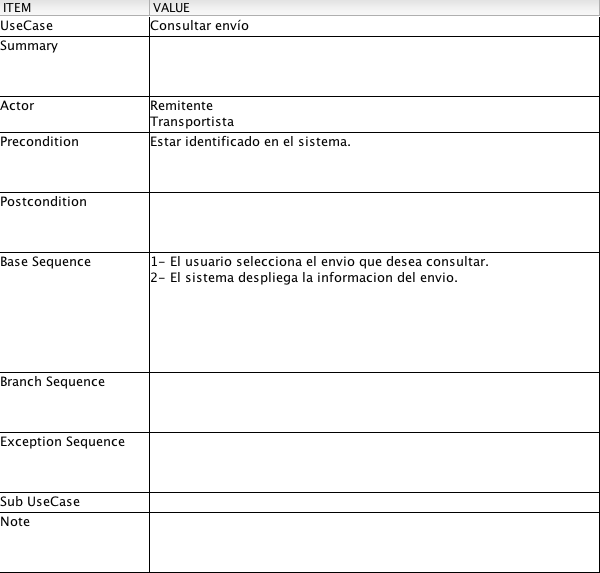
\includegraphics[width=0.75\textwidth]{astah/use_case_consultar_envio.png}
		\end{figure}

		\begin{figure}[H]
			\centering
				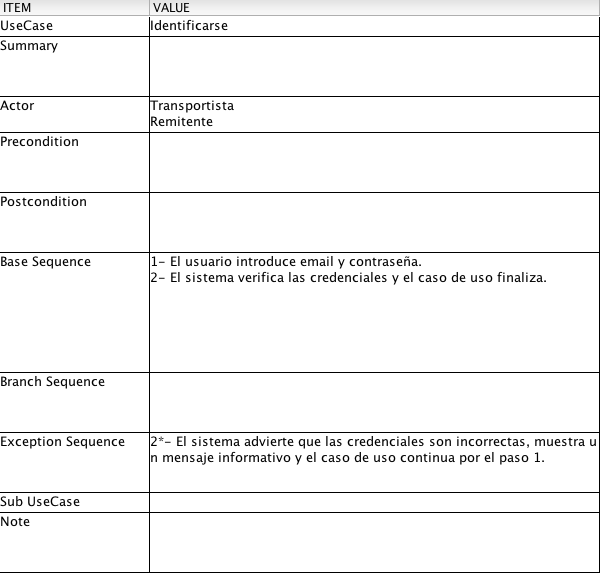
\includegraphics[width=0.75\textwidth]{astah/use_case_identificarse.png}
		\end{figure}

		\begin{figure}[H]
			\centering
				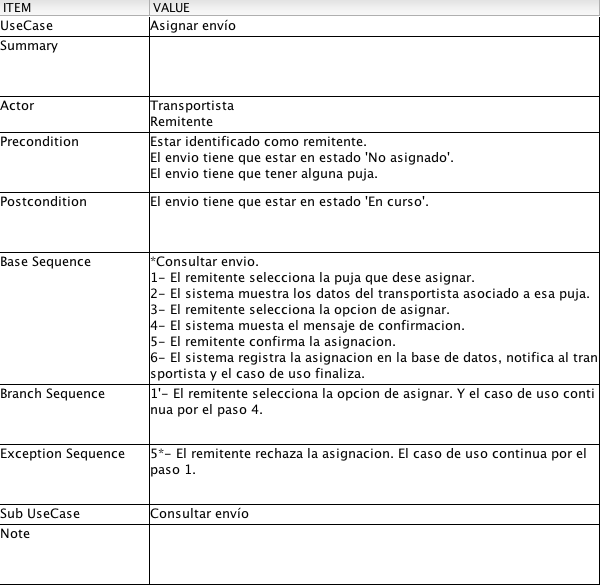
\includegraphics[width=0.75\textwidth]{astah/use_case_asignar_envio.png}
		\end{figure}

		\begin{figure}[H]
			\centering
				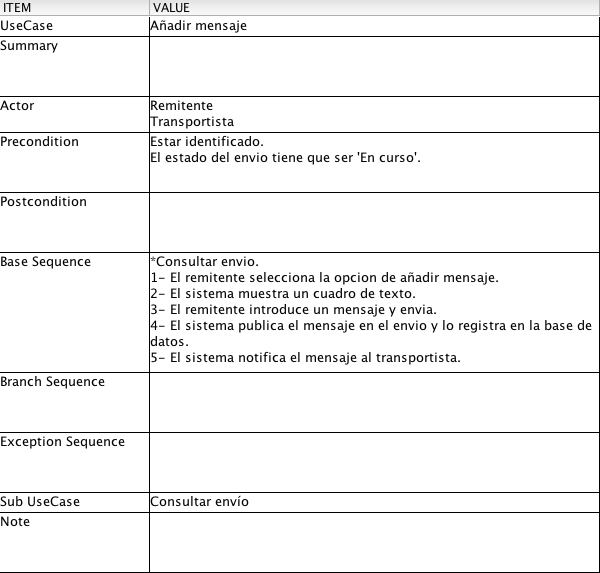
\includegraphics[width=0.75\textwidth]{astah/use_case_anadir_mensaje.png}
		\end{figure}

		\begin{figure}[H]
			\centering
				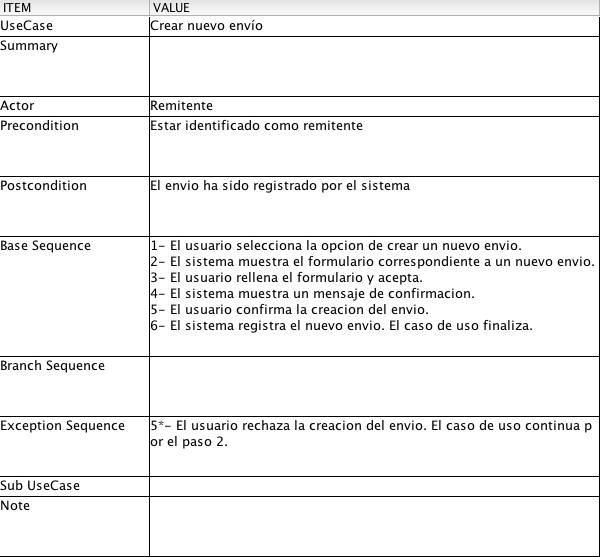
\includegraphics[width=0.75\textwidth]{astah/use_case_crear_envio.png}
		\end{figure}

		\begin{figure}[H]
			\centering
				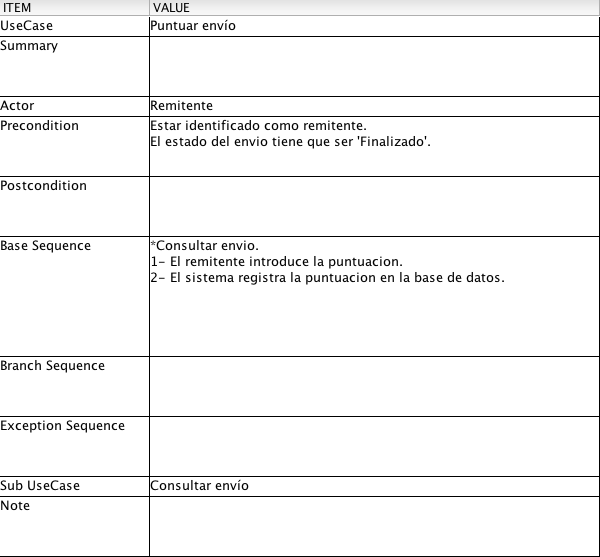
\includegraphics[width=0.75\textwidth]{astah/use_case_puntuar.png}
		\end{figure}

	\section{Modelo del dominio:}

		\begin{figure}[H]
			\centering
				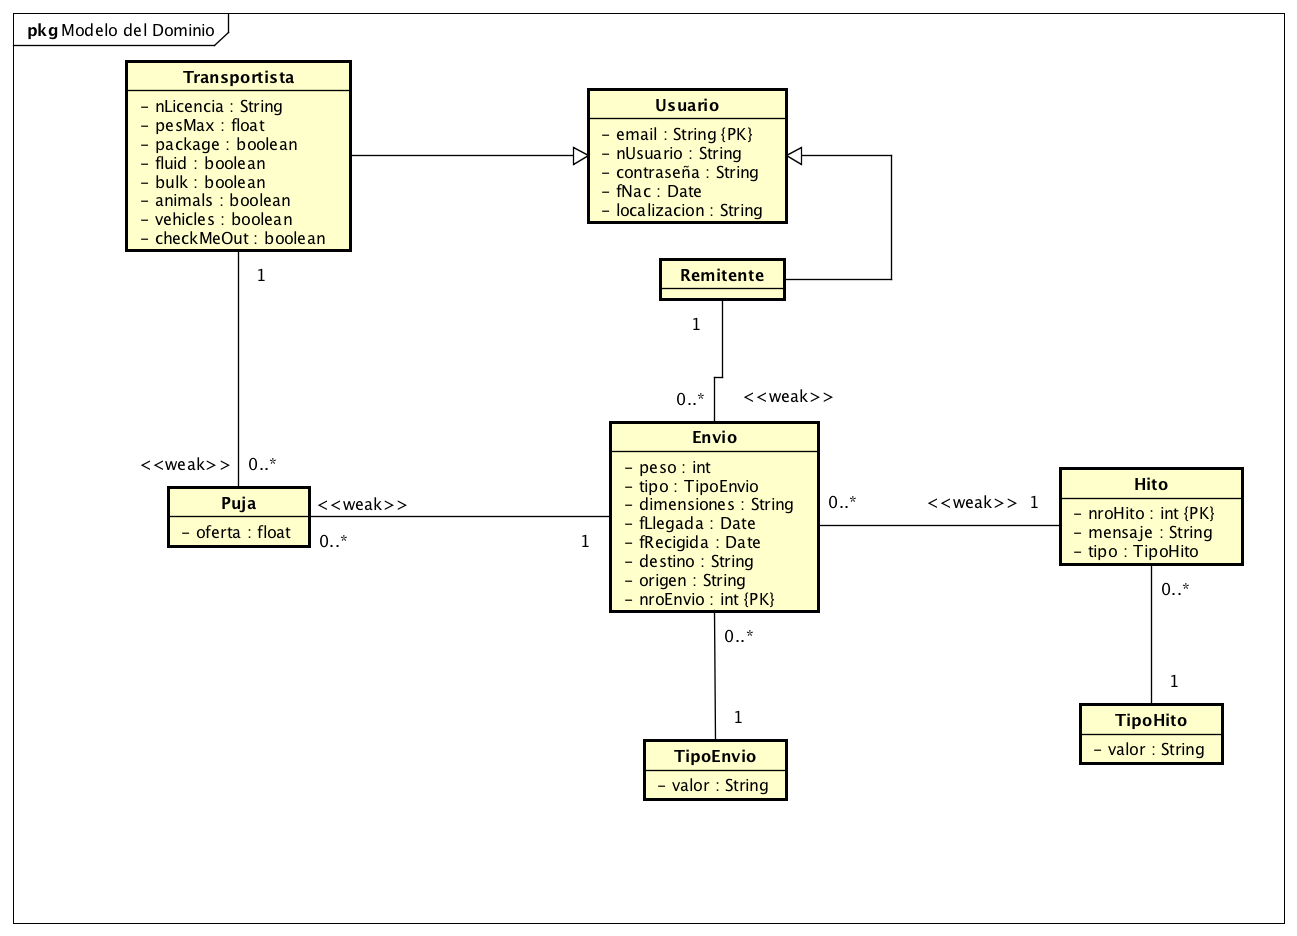
\includegraphics[width=\textwidth]{astah/entidad_relacion.png}
		\end{figure}


	\section{Análisis de los usuarios:}

		\paragraph{}


	\section{Escenarios del sistema futuro:}

		\paragraph{}


\end{document}
